\chapter{Linear Classifiers \& Theory of Error}

{\sf Let's say we have this dataset [pic. 5.1] with two features: a Plus class and a Minus class. If we use some sort of tree algorithm for this, we will get something like this [pic. 5.2]. <...> But ideally we want to separate the dataset with one line [pic. 5.3] (in case of $n$ dimentions it will be the $n-1$ dimentional hyperplane). <...>\\
\begin{figure}[h!]
  \centering
  \begin{subfigure}[l]{0.3\linewidth}
    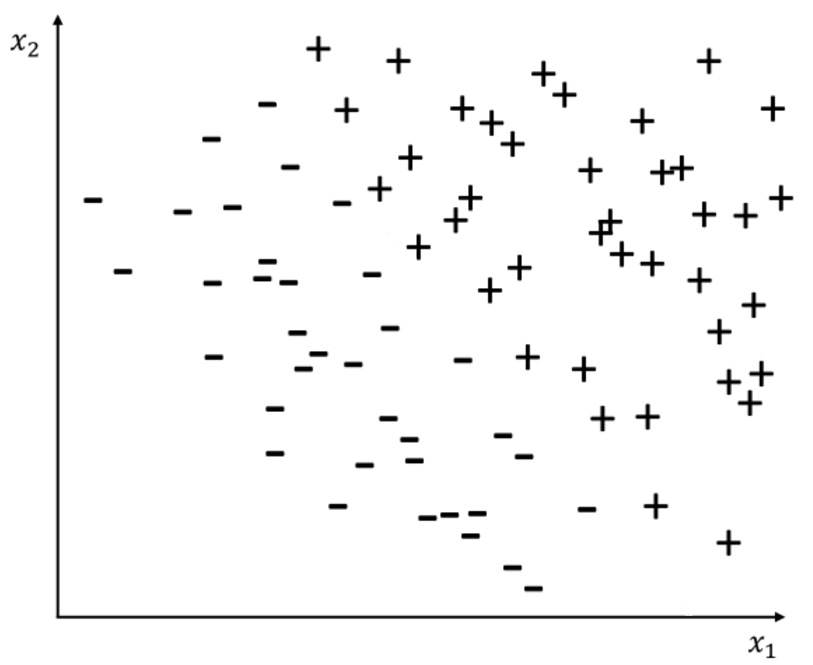
\includegraphics[width=\linewidth]{5a.png}
    \caption*{(5.1) Dataset}
  \end{subfigure}
  \begin{subfigure}[r]{0.3\linewidth}
    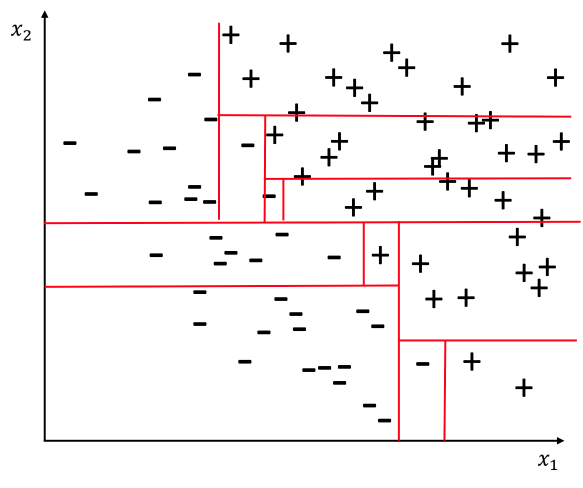
\includegraphics[width=\linewidth]{5b.png}
    \caption*{(5.2) Tree algorithm separating}
  \end{subfigure}
  \begin{subfigure}[r]{0.3\linewidth}
    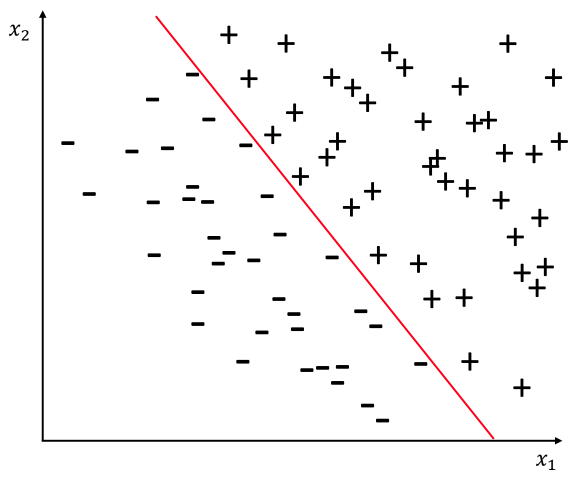
\includegraphics[width=\linewidth]{5c.png}
    \caption*{(5.3) Linear separating}
  \end{subfigure}
\end{figure}
}

\section{Linear Classifiers}

How do we separate? We define the hyperplane and the vector $w$ as the norm vector of that hyperplane and we multiply vector $x$ (from the dataset) by vector $w$. Then we find the threshold. If that\\ multiplication is over the threshold, we will say that $x$ in one class, and if it is under the threshold, $x$ will be in another class.
So this is a hypothesis [$h(x)$ возвращает $-1$ для класса Minus, $1$ для класса Plus]:
$$h(x)=sign\left(\langle w,x\rangle-threshold\right)$$
The one of the algorithms that utilise this hypothesis is called Perceptron.

\subsubsection*{Perceptron}

At the first step we should define a threshold and $w$. The vector $w$ is just a random vector. The threshold can be one of the coefficients of the vector $w$ (for example, $w_0$):
$$h(x)=sign\left(\langle w,x\rangle-w_0\right)$$
Then we can transform each vector $x$ of the dataset to simplify our $h(x)$ function: $$x=(x_1,\ldots,x_d)^T\to(1, x_1, \ldots, x_d)^T$$ After that transformation our hypothesis looks like that:
$$h(x)=sign\left(\langle w, x\rangle\right)=sign(w^Tx)$$
So we start with the random $w$ then we find such point $x$, when our hypothesis $h(x)$ does not match the answer $y$ (in case of two classes the hypothesis can be $1$ or $-1$). And then we just update $w$:
$$w_{new}=w_{old}+yx$$
[В конце концов после нескольких таких итераций мы остановимся. Гиперплоскость, перпендикулярная полученному вектору $w$ будет нашим ответом.]
Why would that work? Expalnation is quite simple: there is a theorem  that proves that it works in case of a linearly separable dataset. {\it <Some intuition about proof of this theorem>} And it actually works and works fast.

\subsubsection*{Pocket Algorithm}

If we have a linearly inseparable case, we have a Pocket Algorithm. {\it <An example with handwritten digits dataset>} A Pocket Algorithm is a simple modification of the Perceptron Algorithm: you just apply it for in given number of iterations and pick the best one in terms of validation dataset. It is called the Pocket Algorithm because you put your values in a pocket: when you find a new minimum you put it in the pocket and then you select the best partition from the pocket.

\subsubsection*{Feature Engineering}

The another way to fight a linearly inseparable dataset is adding new feature. For example [pic.~5.4] you can add feature like distance to (0,0) and get a linearly separable dataset [pic. 5.5].
\begin{figure}[h!]
  \centering
  \begin{subfigure}[l]{0.353\linewidth}
    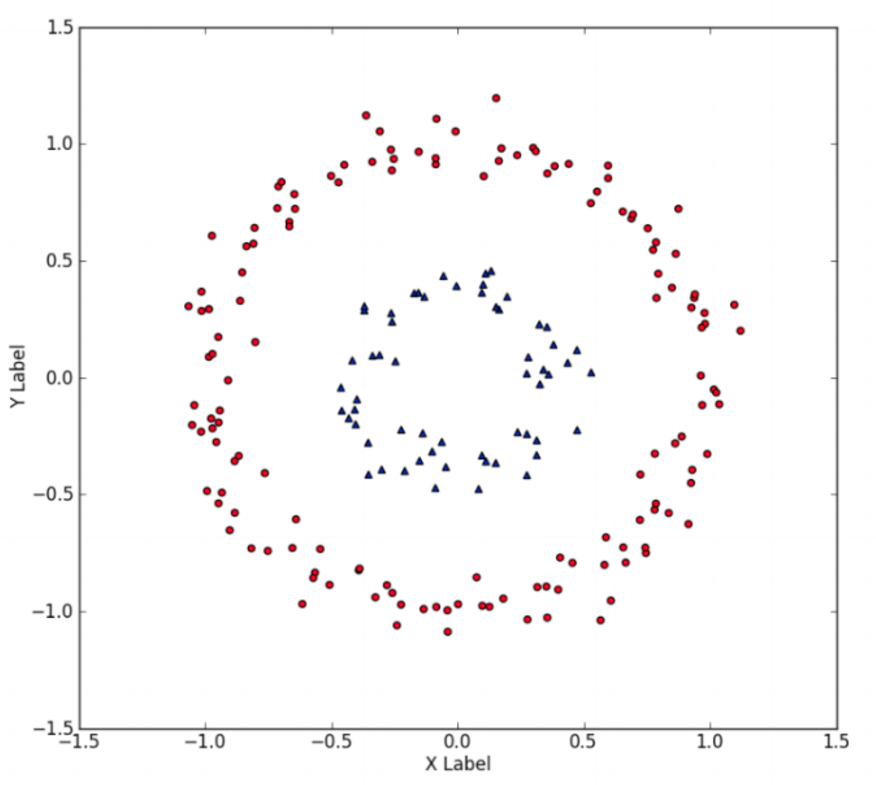
\includegraphics[width=\linewidth]{5d.png}
    \caption*{(5.4) Dataset in $\mathbb{R}^2$}
  \end{subfigure}
  \hspace{2cm}
  \begin{subfigure}[r]{0.4\linewidth}
    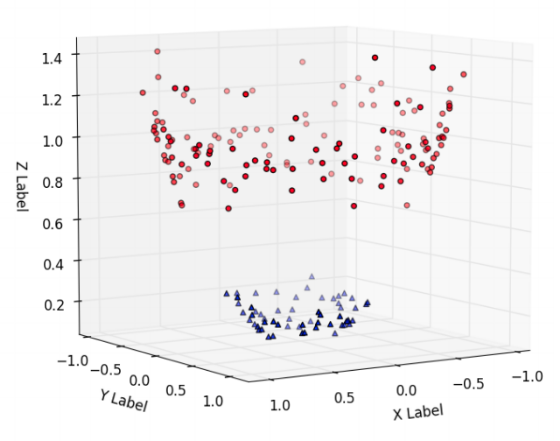
\includegraphics[width=\linewidth]{5e.png}
    \caption*{(5.5) Dataset in $\mathbb{R}^3$}
  \end{subfigure}
\end{figure}

\section{Theory of Error}

However, the problem is how many new features can we add. The more features we have the more overfitting we have.

\subsubsection*{Error in sample and error out of sample}

Let's say we have a dataset with $N$ points ($x_1,\ldots,x_N$), a general set $X$ [которое является абстрактым множеством данных, которые мы хотим классифицировать, например, все люди на Земле и т.д.] and an error function $err$ that somehow defines. An error in sample is
$$E_{in}(h)=\frac{1}{N}\sum\limits_{i=1}^N err(h(x_i),f(x_i))$$
And an error out of sample is
$$E_{out}(h)=E_X[err\left(h(x), f(x)\right)]$$
where $f(x)$ and $h(x)$ returns a class of a point $x$ ($f$ is the target function, $h$ is our hypothesis), $E_{out}$ is the mathematical expectation of our error function on a general set $X$. [$E_{err}$ мы никогда не можем подсчитать напрямую, только оценить. На практике это делается через validation и test датасеты.]\\

\subsubsection*{Hoeffding's inequality}

There is the Hoeffding's inequality:
$$P(|E_{in}(h)-E_{out}(h)|>\varepsilon)\le2e^{-\varepsilon^2N}$$
The difference $E_{in}(h)-E_{out}(h)$ is also called generalization error (sometimes in literature you can found $E_{out}$ as the generalization error). [The generalization error при заданном $h$ -- случайная величина в пространстве датасетов. Неравенство показывает, насколько хорошо ошибки гипотезы $h$ на датасетаx размера $N$ близки к ошибке $h$ на всем множестве $X$.] The big generalization error is a big overfitting and the small generalisation error is a small overfitting.\\
This inequality means for us that if we increase the dataset we exponentialy decrease the probability of overfitting for a one hypothesis. If we have a set of hypotheses then we have to multiply the right side by the $M$ -- number of hypotheses: 
$$P(|E_{in}(h)-E_{out}(h)|>\varepsilon)\le 2Me^{-\varepsilon^2N}$$
[В этом неравенстве $h$ -- лучшая из набора $M$ гипотез. Стоит отметить, что первое неравенство мы применять уже не можем: на разных датасетах лучшая из $M$ гипотез может быть разной.] If $M$ is small we can still guarantee mathematically that increasing the dataset does not get overfitting. Now the problem is how many hypotheses can we have. So this is a graph how our models behave ourselves in terms of complexity:
\begin{figure}[h!]
  \centering
  \begin{subfigure}[l]{0.7\linewidth}
    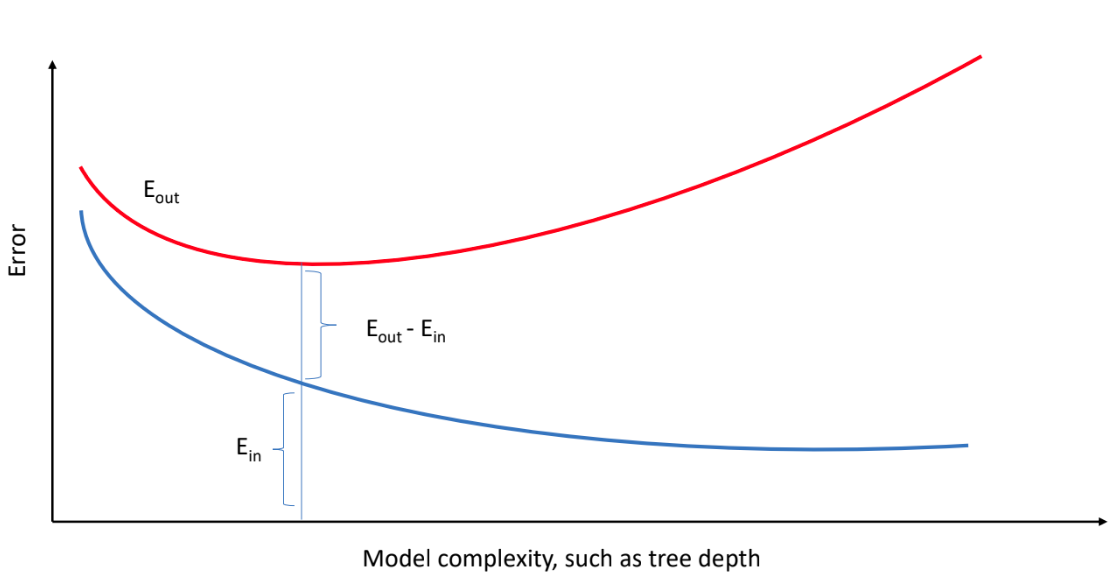
\includegraphics[width=\linewidth]{5f.png}
  \end{subfigure}
\end{figure}

\subsubsection*{From hypotheses to dichotomies}

Hovewer, even in a linear classification you don't have to go through all the hypotheses, for example, if you have some close hypotheses ($|E_{in}(h_1)-E_{out}(h_1)|\approx|E_{in}(h_2)-E_{out}(h_2)|$). So in terms of our math we'll go from hypotheses to dichotomies. The hypothesis is something that is defined for every point of the dataset and the dichotomy is also something that defined for every point of the dataset. But some dichotomies are not possible. [То есть некоторая гипотеза является дихотомией в зависимости от расположения точек из датасета относительно друг друга. К примеру, если вы используете для получения гипотез Perceptron Algorithm, то, чтобы некоторую гипотезу можно было назвать дихотомией, нужно чтобы в этой гипотезе классы были линейно отделимыми. В общем случае дихотомия типа H -- это гипотеза, которую можно получить алгоритмом H]. For example, if you set four points in four corners of the square, you will have only 14 dichotomies, because two dichotomies (where points in one edge have different class) you can not achive with Perceptron Algorithm. The actual number of the dichotomies is called the growth function:
$$m_H(N)=\max\limits_{x_1,\ldots,x_N}|H(x_1,\ldots,x_N)|$$
where $H(x_1,\ldots,x_N)$ is the set of possible dichotomies type $H$ on a points $x_1,\ldots,x_N$, $N$ is the number of points in the dataset. [Стоит понимать, что точки $x_i$ мы берем не из конкретного датасета. Мы берем все возможные расположения точек в пространстве (причем допускаются даже наложения точек друг на друга), считаем для каждого расположения количество возможных дихотомий, а затем берем макимум из подсчитанных значений.]

\subsubsection*{Vapnik-Chervonenkis inequality}

Now we can move from Hoeffding's inequality to Vapnik-Chervonenkis inequality:
$$P(|E_{in}(h)-E_{out}(h)|>\varepsilon)\le m_H(2N)\cdot4e^{-\varepsilon^{1/8}N}$$
The important thing that is now we have number of dichotomies that can be also exponential. And we still can't guarantee that in a big $N$ we will not overfit. However we can prove that the $m_H(2N)$ is almost always polynomial or less. How do we do that? 

\subsubsection*{Proof of polynomiality of a growth function in the presence of a breakpoint}

Well, the growth function is polynomial if it has what we called the breakpoint. The breakpoint is a $\min(k:m_H(k)<2^k)$ [Важно понимать, что для такого $k$ выполняется $\forall n\ge k\colon m_H(n)<2^n$]. In case of four points in 2D space, what we discussed already, $k=4$ is a breakpoint. <...> [Теперь перейдем к доказательству теоремы, используя новое понятие.\\
Пусть у нас есть набор из нескольких бинарных строк длины $N$, записанных в таблицу друг под другом ($i$-й столбец такой таблицы образован набором из $i$-тых символов всех строк). Известно, что для фиксированного $k$ выполнено следующее условие: если выбрать любые $k$ столбцов, то количество различных строк в выбранной части таблицы меньше $2^k$. Определим функцию $B(N,k)$ как наибольшее возможное количество строк в такой таблице.\\
Для начала покажем, что $\forall H\ B(N,k)\ge m_H(N)$, если breakpoint $m_H(N)$ равен $k$. Для этого убедимся, что все дихотомии типа $H$ длины $N$ можно вписать в таблицу с описанным правилом. Действительно, если у такой таблицы выбрать произвольные $k$ столбцов, то полученная таблица состоит из дихотомий длины $k$, значит, количество различных строк в выбранной части равно $m_H(N)<2^k$, что мы и хотели показать.\\
Теперь построим полиномиальную от $N$ оценку сверху на $B(N,k)$, тем самым получив ее и для $m_H(N)$. Для этого возьмем таблицу, удовлетворяющую описанным выше правилом, с наибольшим (т.е. равным $B(N,k)$) количеством строк. Разобьем строки этой таблицы на три части: $\alpha$, $\beta_+$ и $\beta_-$. Первая часть состоит из строк, у которых префикс длины $N-1$ уникален во всей таблице. Во вторую пойдут те из оставшихся, у которых последний символ равен $+1$, в третью, соответственно, $-1$. Таким образом $|\beta_+|=|\beta_-|=:b$. Обозначим $a:=|\alpha|$.\\
\begin{wraptable}{l}{5.8cm}
  \begin{tabular}{|c|c c c c|c|}
    \hline
    \multirow{5}{*}{$\alpha$} & +1 & +1 & $\ldots$ & +1 & +1 \\
                              & +1 & +1 & $\ldots$ & +1 & -1 \\
                              & $\vdots$ & $\vdots$ & $\vdots$ & $\vdots$ & $\vdots$ \\
                              & +1 & -1 & $\ldots$ & -1 & -1 \\
                              & -1 & +1 & $\ldots$ & -1 & +1 \\
    \hline
    \multirow{5}{*}{$\beta_+$}& +1 & -1 & $\ldots$ & +1 & +1 \\
                              & -1 & -1 & $\ldots$ & +1 & +1 \\
                              & $\vdots$ & $\vdots$ & $\vdots$ & $\vdots$& $\vdots$ \\
                              & +1 & -1 & $\ldots$ & +1 & +1 \\
                              & -1 & -1 & $\ldots$ & -1 & +1 \\
    \hline
    \multirow{5}{*}{$\beta_-$}& +1 & -1 & $\ldots$ & +1 & -1 \\
                              & -1 & -1 & $\ldots$ & +1 & -1 \\
                              & $\vdots$ & $\vdots$ & $\vdots$ & $\vdots$  & $\vdots$ \\
                              & +1 & -1 & $\ldots$ & +1 & -1 \\
                              & -1 & -1 & $\ldots$ & -1 & -1 \\
    \hline
  \end{tabular}
\end{wraptable}
Имеем следующее равенство:
$$B(N,k)=a+2b$$
Если мы возьмем префиксы длины $N-1$ строк из $\alpha\cup\beta_+$, то в полученной таблице любые $k$ столбцов образуют не более чем $2^k$ различных строк (поскольку таким свойством удовлетворяла исходная таблица). Значит:  
$$a+b\le B(N-1,k)$$
Теперь выберем префиксы длины $N-1$ строк из $\beta_-$. Заметим, что если в полученной таблице выбрать $k-1$ столбец, то различных строк в выбранной части будет меньше чем $2^{k-1}$ (иначе в исходной таблице столбцы с теми же номерами вместе с $N$-тым содержали бы не менее $2^{k-1}$ различных строк из $\beta_-$ и столько же соответствующих им строк из $\beta_+$, что в сумме дает $2^k$ различных строк, а это невозможно в исходной таблице по построению). Тем самым мы получили:
$$b\le B(N-1,k-1)$$
Суммируя последние два выражения, получаем:
$$B(N,k)=\alpha+2\beta\le B(N-1, k)+B(N-1,k-1)$$
Теперь мы можем показать следующую оценку:
$$B(N,k)\le\sum\limits_{i=0}^{k-1}\binom{N}{i}$$
Знаем, что $B(N,1)=1$, $B(1,k>1)=2$ и $\binom{N-1}{i-1}+\binom{N-1}{i}=\binom{N}{i}$, значит, использую индукцию по $N$ и $k$, можем показать:
$$B(N,k)\le B(N-1,k)+B(N-1,k-1)\le\sum\limits_{i=0}^{k-1}\binom{N-1}{i}+\sum\limits_{i=0}^{k-2}\binom{N-1}{i}=$$ $$=1+\sum\limits_{i=1}^{k-1}\binom{N-1}{i}+\sum\limits_{i=1}^{k-1}\binom{N-1}{i-1}=1+\sum\limits_{i=1}^{k-1}\binom{N}{i}=\sum\limits_{i=0}^{k-1}\binom{N}{i}$$
Последняя сумма является многочленом от $N$.]

\subsubsection*{VC-dimention}

$d_{VC}(H)$ for hypotheses type $H$ is the maximum number $N$ such that $m_H(N)=2^N$. If $k$ is the breakpoint, $d_{VC}=k-1$, so:
$$m_H(N)\le B(N,k)\le\sum\limits_{i=0}^{k-1}\binom{N}{i}=\sum\limits_{i=0}^{d_{VC}}\le N^{d_{VC}}+1$$
Why is this important? Because we can pull that in the Vapnik-Chervonenkis inequality and guarantee that we don't overfit in a big dataset. And the number $d_{VC}$ shows the effective complexity of a model.

\subsubsection*{VC-dimention for perceptron}

Now we prove that if $d$ is the space dimensionality, $d_{VC}=d+1$ [для случая, когда классы в дихотомии линейно разделимы].\\
So we have $d$ dimentions and at first we prove that we can have all the posible dichotomies for $d+1$ points. Let's construct the set of these points [не забываем добавить $d+1$'ую размерность, координата которой у всех точек из датасета равна 1]:
$$X=
\begin{pmatrix}
  x_1^T \\
  x_2^T \\
  x_3^T \\
  \ldots \\
  x_{d+1}^T
\end{pmatrix}
=
\begin{pmatrix}
  1 & 0 & 0 & 0 & \ldots & 0 \\
  1 & 1 & 0 & 0 & \ldots & 0 \\
  1 & 0 & 1 & 0 & \ldots & 0 \\
    &   &   & \vdots \\
  1 & 0 & 0 & 0 & \ldots & 1
\end{pmatrix}
$$
And we get invertable matrix, so we can solve this [обозначения как в описании Perceptron Algorithm: $y$ -- классы точек, $w$ -- нормаль к гиперплоскости, которую мы ищем]:
$$sign(Xw)=y;$$
$$Xw=y;$$
$$w=X^{-1}y.$$
Now we only need to prove that we can't have all hypotheses as dichotomies in $d+2$ points. So let's take $x_1,\ldots,x_{d+1},x_{d+2}$.  If two points from them are the same we already can't have all dichotomies. If there's not same points, let's assume that all hypotheses on that points are dichotomies. Because we work in $d+1$ dimentional space [$d+1$'ая размерность -- та, которая состоит из едениц] there is a vector $x_j$ that can be expressed to a linear combination of other $d+1$ vectors:
$$x_j=\sum\limits_{i\ne j}a_ix_i;$$
$$y_j=sign(w^Tx_j)=sign\left(\sum\limits_{i\ne j}a_iw^Tx_i\right).$$
If $y_i=sign(a_i)$ the $y_j$ can't be $-1$ (because $\forall i\ne j\ a_iw^Tx_i$ is always positive [так как $a_i$ и $w^Tx_i$ одного знака, поскольку мы так определили $y_i$]), so our assumption is incorrect and we prove the theorem.

\subsubsection*{Sufficient data}

So we proved that for perecptron algorithm:

$$P(|E_{in}(h)-E_{out}(h)|>\varepsilon)\le m_H(2N)\cdot4e^{-\varepsilon^{1/8}N}\approx N^{d_{VC}}e^{-N}$$

What does that give us? Well, if you want a nice hypothesis and if you don't want overfit you'd better have sufficient data: when $N\ge 10d_{VC}$ everything is OK. The problem is how to get the $d_{VC}$. For perceptron we have already get, for neural network we can calculate $d_{VC}$ as well because we can find the breakpoint. And what we do in the real world is the validation.

\section{Validation}

[Валидация -- процесс подбора оптимальных параметров обучающего алгоритма, используя заранее подготовленную для этого выборку. В отличие от валидации, тестирование и тестирующая выборка из датасета нужны для сравнения работы разных алгоритмов.]\\
Why is validation work? It works because dichotomy inequality works in it's original form, because we train our hypotheses on our dataset. So the validation is just pass the best hypothesis. There is an inequality for one hypothesis:
$$P(|E_{val}(h)-E_{out}(h)|>\varepsilon)\le2e^{-\varepsilon^2N}$$
Now the problem is: if you have many various parameters and so on then if you start pasting many hypotheses to your validation dataset you have to multiply right side by the number of hypotheses. That is why we go from validation to testing. That is why we train, validate and test. Because of Hoeffding's inequality. So you train on train dataset then you pass your answer on your validation dataset and you estimate the overfitting. The proper validation size is $K=\frac{N}{5}$ ($N$ is number of points in your dataset).

\subsubsection*{Cross-validation}

The problem with validation is we don't use all points. The validation dataset has only $20\%$ of all points and we don't use that points in our training. That is bad, because points are usualy expensive: you spend money for each point you have. So we do want to use them all. The thing what helps us is caled cross-validation.\\
The cross validation is the way to use all the points. We separate all dataset on 10 datasets, and take one of them as a validation dataset and all the others as a training dataset. And repeat. Now we should talk about data leaking.

\subsubsection*{Data leaking}

%Let's imagine you have a EEG signal from five pacients and you need to predict an epileptic seizure. The signals looks like this:\\
%{\it <One day there will be a pic>}\\
%And at some points in the EEG you have an epileptic seizures. You can say: Ok, let's have the validation dataset, let's have a trainig dataset. But you can divide your EEG diagrams like this:\\
%{\it <One day there will be a pic>}\\
%<...> What polutes your dataset. So you should divide like this:\\
%{\it <One day there will be a pic>}\\
{\it <Examples with EEG and MRT>}

\subsubsection*{Train $\rightarrow$ Validate $\rightarrow$ Test}

\begin{enumerate}[label=$\bullet$]
  \item Train the algorithm on your train dataset.
  \item Optimize hyperparameters on validation (or crossvalidation).
  \item Check the final perfomance on test.
\end{enumerate}